
\chapter{Differentiation}

 
%25. 
\section{Introduction}

We shall now proceed to investigate the manner in which 
a function changes in value as the independent variable 
changes. The fundamental problem of the Differential Calculus 
is to establish a measure of this change in the function with 
mathematical precision. It was while investigating problems of 
this sort, dealing with continuously varying quantities, that 
Newton\footnote{Sir Isaac Newton (1642-1727), an Englishman, 
was a man of the most extraordinary genius. He developed the 
science of the Calculus under the name of Fluxions. Although 
Newton had discovered and made use of the new science as 
early as 1670, his first published work in which it occurs 
is dated 1687, having the title {\bf Philosophiae Naturalis 
Principia Mathematica}. This was Newton's principal work. 
Laplace said of it, ``It will always remain preminent above 
all other productions of the human mind.'' See frontispiece.}
was led to the discovery of the fundamental principles 
of the Calculus, the most scientific and powerful tool of the 
modern mathematician.

%26. 
\section{Increments}
The {\it increment} of a variable in changing from one 
numerical value to another is the difference found by 
subtracting the first value from the second. An increment of $x$ 
is denoted by the symbol $\Delta x$, read ``delta $x$''.
\index{increment}

The student is warned against reading this symbol 
``delta times $x$'', it having no such meaning. Evidently 
this increment may be either positive or negative\footnote{Some 
writers call a negative increment a decrement.}
according as the variable in changing is increasing or 
decreasing in value. Similarly,

\qquad     $\Delta y$ 	denotes an increment of $y$,

\qquad    $\Delta \phi$ 	denotes an increment of $\phi$,

\qquad  $\Delta f(x)$ 	denotes an increment $f(x)$, etc.

If in $y = f(x)$ the independent variable $x$, takes on an increment 
$\Delta x$, then $\Delta y$ is always understood to denote the 
corresponding increment of the function $f(x)$ (or dependent variable $y$).

The increment $\Delta y$ is always assumed to be reckoned 
from a definite initial value of $y$ corresponding to the arbitrarily 
fixed initial value of $x$ from which the increment $\Delta x$ 
is reckoned. 

\begin{example}
{\rm
For instance, consider the function

\[
    y = x^2. 
\]
Assuming $x = 10$ for the initial value of $x$ fixes $y = 100$ as 
the initial value of $y$.
Suppose $x$ increases to $x = 12$, that is, $\Delta x 	= 2$;
then $y$ increases to $y = 144$, and $\Delta y 	= 44$.
Suppose $x$ decreases to $x = 9$, that is, $\Delta x = - 1$;
then $y$ increases to $y= 81$,	and $\Delta y 	= - 19$.
}
\end{example}

It may happen that as $x$ increases, $y$ decreases, or the reverse; 
in either case $\Delta x$ and $\Delta y$ will have opposite signs.

It is also clear (as illustrated in the above example) that if 
$y = f(x)$ is a continuous function and $\Delta x$ is decreasing in 
numerical value, then $\Delta y$ also decreases in numerical value.


%27
\section{Comparison of increments}
Consider the function

\[
%(A)
 y = x^2.
\]
Assuming a fixed initial value for $x$, let $x$ take on an 
increment $\Delta x$. Then $y$ will take on a corresponding 
increment $\Delta y$, and we have

\[
 	y + \Delta y 	= (x + \Delta x)^2,
\]
or, 

\[
	y + \Delta y 	= x^2+ 2x \cdot \Delta x + (\Delta x)^2.
\]
Subtracting $y 	= x^2$ 
from this, % new

\begin{equation}
%(B)
\Delta y = 2x \cdot \Delta x + (\Delta x)^2,
\label{eqn:B-IV}
\end{equation}
we get the increment $\Delta y$ in terms of $x$ and $\Delta x$.
To find the ratio of the increments, divide 
%(B) 
(\ref{eqn:B-IV})  % new
by $\Delta x$, giving

\[
    \frac{\Delta y}{\Delta x} = 2x + \Delta x.
\]
If the initial value of $x$ is $4$, it is evident that

\[
    \lim_{\Delta x \to 0} \frac{\Delta y}{\Delta x} = 8. 
\]
Let us carefully note the behavior of the ratio of the increments 
of $x$ and $y$ as the increment of $x$ diminishes.

\vskip .2in

{\small{
\begin{tabular}{lllllll}
Initial      &      New        &  Increment   &  Initial  &   New   &   Increment       &    \\
value of $x$ &    value of $x$ &  $\Delta\, x$ & value of $y$ & value of $y$ & $\Delta\, y$ & $\frac{\Delta y}{\Delta x}$ \\ \hline
4 &	5.0 &	1.0 &	16 &	25.     & 9.   & 9.  \\
4 &	4.8 &	0.8 &	16 &	23.04   & 7.04 & 8.8  \\
4 &	4.6 &	0.6 &	16 &	21.16   & 5.16 & 8.6  \\
4 &	4.4 &	0.4 &	16 &	19.36   & 3.36 & 8.4  \\
4 &	4.2 &	0.2 &	16 &	17.64   & 1.64 & 8.2  \\
4 &	4.1 &	0.1 &	16 &	16.81   & 0.81 & 8.1  \\
4 &	4.01 &	0.01 &	16 &	16.0801 & 0.0801 &8.01  \\
\end{tabular}
}}
\vskip .2in

\noindent
It is apparent that as $\Delta\, x$ decreases, $\Delta\, y$ also diminishes, 
but their ratio takes on the successive values $9$, $8.8$, $8.6$, $8.4$, $8.2$, $8.1$, $8.01$; 
illustrating the fact that $\frac{\Delta y}{\Delta x}$ can be brought as near to $8$ 
in value as we please by making $\Delta\, x$ small enough. Therefore\footnote{The 
student should guard against the common error of concluding that because the 
numerator and denominator of a fraction are each approaching zero as a limit, 
the limit of the value of the fraction (or ratio) is zero. The limit of the 
ratio may take on any numerical value. In the above example the limit is $8$.},

\[
    \lim_{\Delta x \to 0} \frac{\Delta y}{\Delta x} = 8. 
\]

%28. 
\section{Derivative of a function of one variable}

The fundamental definition of the Differential Calculus is:

\begin{definition}
{\rm
The {\it derivative}\footnote{Also called the differential coefficient or the derived function.} 
of a function is the limit of the ratio 
of the increment of the function to the increment of the independent 
variable, when the latter increment varies and approaches the limit zero.
}
\end{definition}
\index{derivative}

When the limit of this ratio exists, the function is said to be 
{\it differentiable}, or to {\it possess a derivative}.
\index{differentiable}


The above definition may be given in a more compact form 
symbolically as follows: Given the function

\begin{equation}
%(A) 
y = f(x),
\label{eqn:A-28}
\end{equation}
and consider $x$ to have a fixed value.

Let $x$ take on an increment $\Delta\, x$; then the function $y$ takes on an 
increment $\Delta\, y$, the new value of the function being

\begin{equation}
%(B) 
y + \Delta\, y = f(x + \Delta\, x).
\label{eqn:B-28}
\end{equation}
To find the increment of the function, subtract %(A) from (B)
(\ref{eqn:A-28}) from (\ref{eqn:B-28}), % new 
giving

\[
%(C) 
\Delta\, y = f(x + \Delta\, x) - f(x).
\]
Dividing by the increment of the variable, $\Delta\, x$, we get

\begin{equation}
%(D) 
\frac{\Delta y}{\Delta x} = \frac{f(x + \Delta x) - f(x)}{\Delta x}.
\label{eqn:D-28}
\end{equation}
The limit of this ratio when $\Delta\, x$ approaches the limit 
zero is, from our definition, the derivative and is denoted 
by the symbol $\frac{dy}{dx}$.
\index{$\frac{dy}{dx}$}
Therefore

\[
%(E) 
\frac{dy}{dx} = \lim_{\Delta x \to 0} \frac{f(x + \Delta x) - f(x)}{\Delta x}.
\]
defines the {\it derivative of $y$ [or $f(x)$] with respect to $x$}.
From % (D)
(\ref{eqn:B-28}), % new 
we also get

\[
    \frac{dy}{dx} = \lim_{\Delta x \to 0} \frac{\Delta y}{\Delta x}
\]
The process of finding the derivative of a function is called {\it differentiation}.
\index{differentiation}

It should be carefully noted that the derivative is the limit of the 
ratio, not the ratio of the limits. The latter ratio would assume the 
form $\frac{0}{0}$, which is indeterminate (\S \ref{sec:14}).


%29. 
\section{Symbols for derivatives}

Since $\Delta\, y$ and $\Delta\, x$ are always finite and have 
definite values, the expression

\[
    \frac{\Delta y}{\Delta x}
\]
is really a fraction. The symbol

\[
    \frac{dy}{dx},
\]
however, is to be regarded not as a fraction but as the limiting value 
of a fraction. In many cases it will be seen that this symbol does 
possess fractional properties, and later on we shall show how meanings 
may be attached to $dy$ and $dx$, but for the present the symbol $\frac{dy}{dx}$ 
is to be considered as a whole.

Since the derivative of a function of $x$ is in general also a function of $x$, 
the symbol $f'(x)$ is also used to denote the derivative of $f(x)$.

Hence, if $y 	= f(x)$,
we may write $\frac{dy}{dx} = f'(x)$,
which is read ``the derivative of $y$ with respect to $x$ equals $f$ prime of $x$.'' 
The symbol

\[
    \frac{d}{dx}
\]
when considered by itself is called the {\it differentiating operator}, 
and indicates that any function written after it is to be differentiated with 
respect to $x$. 
\index{differentiating operator}
Thus

\qquad   $ \frac{dy}{dx}$ or $\frac{d}{dx} y$ indicates the derivative of $y$ with respect to $x$;

\qquad  $ \frac{d}{dx} f(x)$ indicates the derivative of $f(x)$ with respect to $x$;

\qquad $\frac{d}{dx} (2x^2 + 5)$ indicates the derivative of $2x^2 + 5$ with respect to $x$;

\qquad $ y'$ is an abbreviated form of $\frac{dy}{dx}$.

 
The symbol $D_x$ is used by some writers instead of $\frac{d}{dx}$. If then
\[
   y = f(x),
\]
we may write the identities

\[
    y' = \frac{dy}{dx} = \frac{d}{dx} y = D_x f(x) = f'(x).
\]


%30. 
\section{Differentiable functions}

From the Theory of Limits 
(Chapter \ref{ch:3}) % new
it is clear that if the derivative of a 
function exists for a certain value of the independent variable, the 
function itself must be continuous for that value of the variable.

The converse, however, is not always true, functions having been 
discovered that are continuous and yet possess no derivative. But such 
functions do not occur often in applied mathematics, and in this book only 
differentiable functions are considered, that is, functions that possess a 
derivative for all values of the independent variable save at most for isolated values.

%31. 
\section{General rule for differentiation}
\label{sec:31}

From the definition of a derivative it is seen that the process of 
differentiating a function $y = f(x)$ consists in taking the following 
distinct steps:


{\bf General rule for differentiating}\footnote{Also called the 
Four-step Rule.}:

\begin{itemize}

\item
FIRST STEP. In the function replace $x$ by $x + \Delta\, x$, giving a new 
value of the function, $y + \Delta\, y$.

\item
SECOND STEP. Subtract the given value of the function from the new value 
in order to find $\Delta\, y$ (the increment of the function).

\item
THIRD STEP. Divide the remainder $\Delta\, y$ (the increment of the 
function) by $\Delta\, x$ (the increment of the independent variable).

\item
FOURTH STEP. Find the limit of this quotient, when $\Delta\, x$ 
(the increment of the independent variable) varies and approaches the 
limit zero. This is the derivative required.
\end{itemize}

The student should become thoroughly familiar with this rule by applying 
the process to a large number of examples. Three such examples will now be 
worked out in detail.

\begin{example}
{\rm
Differentiate $3x^2 + 5$.

Solution. Applying the successive steps in the General Rule, we get, 
after placing

\[
  	y 	= 3x^2 + 5,
\]
First step. 

\[
y + \Delta\, y 	= 3(x + \Delta\, x)2 + 5
  	= 3x^2 + 6x \cdot \Delta x + 3(\Delta x)^2 + 5.
\]
Second step.
\[
\begin{array}{ll}
y + \Delta\, y &	= 3x^2 + 6 x \cdot \Delta x + 3(\Delta x)^2 	+ 5\\
y &	= 3x^2 	+ 5\\
\Delta\, y &	= 6x \cdot \Delta x + 3(\Delta x)^2. 
\end{array}
\]	 
Third step. $	\frac{\Delta y}{\Delta x} 	= 6x + 3 \cdot \Delta x.$

\noindent
Fourth step. 	$\frac{dy}{dx} 	= 6x$.   
We may also write this
\[
    \frac{d}{dx} (3x^2 + 5) = 6x. 
\]

Here's how to use \sage to verify this (for simplicity, we set $h=\Delta x$):

\vskip .2in

\begin{Verbatim}[fontsize=\scriptsize,fontfamily=courier,fontshape=tt,frame=single,label=\sage]

sage: x = var("x")
sage: h = var("h")
sage: f(x) = 3*x^2 + 5
sage: Deltay = f(x+h)-f(x)
sage: (Deltay/h).expand()
6*x + 3*h
sage: limit((f(x+h)-f(x))/h,h=0)
6*x
sage: diff(f(x),x)
6*x

\end{Verbatim}

\vskip .1in
\noindent
}
\end{example}

\begin{example}
{\rm
Differentiate $x^3 - 2x + 7$.

Solution. Place $y 	= x^3 - 2x + 7$.

\noindent
First step. 

\[
\begin{array}{ll}
	y + \Delta y &	= (x + \Delta x)3 - 2(x + \Delta x) + 7\\
   &	= x^3 	+ 3x^2 \cdot \Delta x + 3x \cdot (\Delta x)^2 + (\Delta x)^3 	- 2x 	- 2 \cdot \Delta x 	+ 7
\end{array}
\]
Second step. 
\[
\begin{array}{ll}
y + \Delta y &	= x^3 	+ 3x^2 \cdot \Delta x + 3x \cdot (\Delta x)^2 + (\Delta x)^3 - 2x - 2 \cdot \Delta x 	+ 7\\
y &= x^3 - 2x 	  	+ 7\\
\Delta y &	= 	3x^2 \cdot \Delta x + 3x \cdot (\Delta x)^2 + (\Delta x)^3 - 2 \cdot \Delta x 
\end{array}
\]	 
Third step. $\frac{\Delta y}{\Delta x} 	= 3x^2 + 3x \cdot \Delta x + (\Delta x)^2 - 2$.

\noindent
Fourth step. $\frac{dy}{dx} 	= 3x^2 - 2$.
Or, 	
\[
\frac{d}{dx} (x^3 - 2x + 7) 	= 3x^2 - 2.
\]
}
\end{example}

\begin{example}
{\rm
Differentiate $\frac{c}{x^2}$.

Solution. Place $y = \frac{c}{x^2}$.

\noindent
First step. $	y + \Delta y 	= \frac{c}{(x + \Delta x)^2}$.

\noindent
Second step. 
\[
\begin{array}{ll}
	y + \Delta y &	= \frac{c}{(x + \Delta x)^2}\\
  	y \qquad &	= \frac{c}{x^2}\\
  	\Delta y &	= \frac{c}{(x + \Delta x)^2} - \frac{c}{x^2} = \frac{-c \cdot \Delta x(2x + \Delta x)}{x^2(x + \Delta x)^2}.
\end{array}
\]
Third step. $	\frac{\Delta y}{\Delta x} 	= -c \cdot \frac{2x + \Delta x}{x^2(x + \Delta x)^2}$.

\noindent
Fourth step. $	\frac{dy}{dx} 	= -c \cdot \frac{2x}{x^2(x)^2} 	= -\frac{2c}{x^3}$.
Or, $\frac{d}{dx} \left ( \frac{c}{x^2} \right ) = 	\frac{-2c}{x^3}$.
}
\end{example}


\section{Exercises}

Use the General Rule, %p. 29 [§ 31], 
\S \ref{sec:31} % new
in differentiating the following functions:
\vskip .2in

%\begin{tabular}{lll}
\begin{enumerate}

%Given function &  & Selected answers \\ \hline
% & & \\
\item
%1. 
$y 	= 3x^2$ %& \qquad  \qquad \qquad\qquad\qquad\qquad \qquad \qquad &

Ans: $\frac{dy}{dx} 	= 6x$
%\\ 
% & &  \\

\item
%2. 
$y 	= x^2 + 2$ %& \qquad  \qquad \qquad\qquad\qquad\qquad \qquad \qquad & 

Ans: $\frac{dy}{dx} 	= 2x$
%\\
% & &  \\

\item
%3. 
$y 	= 5 - 4x$ %& \qquad  \qquad \qquad\qquad\qquad\qquad \qquad \qquad &

Ans: $\frac{dy}{dx} 	= - 4$
%\\
% & &  \\

\item
%4. 
$s 	= 2t^2 - 4$ %& \qquad  \qquad \qquad\qquad\qquad\qquad \qquad \qquad & 

Ans:	$\frac{ds}{dt} 	= 4t$
%\\
% & &  \\

\item
%5. 
$y 	= \frac{1}{x}$ %& \qquad  \qquad \qquad\qquad\qquad\qquad \qquad \qquad &  

Ans:$\frac{dy}{dx} 	= -\frac{1}{x^2}$
%\\
% & &  \\

\item
%6.
$ y 	= \frac{x + 2}{x}$ %& \qquad  \qquad \qquad\qquad\qquad\qquad \qquad \qquad & 	

Ans: $\frac{dy}{dx} 	= -\frac{-2}{x^2}$
%\\
% & &  \\

\item
%7. 
$y 	= x^3$ %& \qquad  \qquad \qquad\qquad\qquad\qquad \qquad \qquad &  

Ans: $\frac{dy}{dx} 	= 3x^2$
%\\
% & &  \\

\item
%8. 
$y = 2x^2 - 3$ %& \qquad  \qquad \qquad\qquad\qquad\qquad \qquad \qquad &  

Ans: $\frac{dy}{dx} = 4x$
%\\
% & &  \\

\item
%9. 
$y 	= 1 - 2x^3$ %& \qquad  \qquad \qquad\qquad\qquad\qquad \qquad \qquad &  

Ans: $\frac{dy}{dx} 	= -6x^2$
%\\
% & &  \\

\item
%10. 
$\rho 	= a\theta^2$ %& \qquad  \qquad \qquad\qquad\qquad\qquad \qquad \qquad & 

Ans: $\frac{d\rho}{d\theta} 	= 2a\theta$
%\\
% & &  \\

\item
%11. 
$y 	= \frac{2}{x^2}$ %& \qquad  \qquad \qquad\qquad\qquad\qquad \qquad \qquad & 

Ans: $\frac{dy}{dx} 	= -\frac{4}{x^3}$
%\\
% & &  \\

\item
%12. 
$y 	= \frac{3}{x^2 - 1}$ %& \qquad  \qquad \qquad\qquad\qquad\qquad \qquad \qquad & 

Ans: $\frac{dy}{dx} 	= -\frac{6x}{(x^2 - 1)^2}$
%\\
% & &  \\

Here's how to use \sage to verify this:

\vskip .2in

\begin{Verbatim}[fontsize=\scriptsize,fontfamily=courier,fontshape=tt,frame=single,label=\sage]

sage: y = 3/(x^2-1)
sage: diff(y,x)
-6*x/(x^4 - 2*x^2 + 1)

\end{Verbatim}

\item
%13. 
$y = 7x^2 + x$  %& \qquad  \qquad \qquad\qquad\qquad\qquad \qquad \qquad & \\
% & &  \\

\item
%14. 
$s = at^2 - 2bt$  %& \qquad  \qquad \qquad\qquad\qquad\qquad \qquad \qquad & \\
% & &  \\

\item
%15. 
$r = 8t + 3t^2$ %& \qquad  \qquad \qquad\qquad\qquad\qquad \qquad \qquad & \\
% & &  \\

\item
%16. 
$y = \frac{3}{x^2}$ %& \qquad  \qquad \qquad\qquad\qquad\qquad \qquad \qquad & \\
% & &  \\

\item
%17. 
$s = -\frac{a}{2t + 3}$ %& \qquad  \qquad \qquad\qquad\qquad\qquad \qquad \qquad & \\
% & &  \\

\item
%18. 
$y = bx^3 - cx$ %& \qquad  \qquad \qquad\qquad\qquad\qquad \qquad \qquad & \\
% & &  \\
%\end{tabular}
%\newpage

%\begin{tabular}{lll}

%Given function &  & Selected answers \\ \hline

\item
%19. 
$\rho = 3\theta^3 - 2\theta^2$ %& \qquad  \qquad \qquad\qquad\qquad\qquad \qquad \qquad & \\
% & &  \\

\item
%20. 
$y = \frac{3}{4}x^2 - \frac{1}{2}x$ %& \qquad  \qquad \qquad\qquad\qquad\qquad \qquad \qquad &\\ 
% & &  \\

\item
%21. 
$y = \frac{x^2 - 5}{x}$ %& \qquad  \qquad \qquad\qquad\qquad\qquad \qquad \qquad & \\
% & &  \\

\item
%22. 
$\rho = \frac{\theta^2}{1 + \theta}$ %& \qquad  \qquad \qquad\qquad\qquad\qquad \qquad \qquad &\\ 
% & &  \\

\item
%23. 
$y = \frac{1}{2}x^2 + 2x$ %& \qquad  \qquad \qquad\qquad\qquad\qquad \qquad \qquad & \\
% & &  \\

\item
%24. 
$z = 4x - 3x^2$ %& \qquad  \qquad \qquad\qquad\qquad\qquad \qquad \qquad & \\
% & &  \\

\item
%25. 
$\rho = 3\theta + \theta^2$ %& \qquad  \qquad \qquad\qquad\qquad\qquad \qquad \qquad & \\
% & &  \\

\item
%26. 
$y = \frac{ax + b}{x^2}$ %& \qquad  \qquad \qquad\qquad\qquad\qquad \qquad \qquad & \\
% & &  \\

\item
%27. 
$z = \frac{x^3 + 2}{x}$ %& \qquad  \qquad \qquad\qquad\qquad\qquad \qquad \qquad & \\
% & &  \\

\item
%28. 
$y 	= x^2 - 3x + 6$ %& \qquad  \qquad \qquad\qquad\qquad\qquad \qquad \qquad &  

Ans: $y' 	= 2x - 3$
%\\
% & &  \\

\item
%29. 
$s 	= 2t^2 + 5t - 8$ %& \qquad  \qquad \qquad\qquad\qquad\qquad \qquad \qquad &  

Ans: $s' 	= 4t + 5$
%\\
% & &  \\
Here's how to use \sage to verify this (for simplicity, we set $h=\Delta t$):

\vskip .2in

\begin{Verbatim}[fontsize=\scriptsize,fontfamily=courier,fontshape=tt,frame=single,label=\sage]

sage: h = var("h")
sage: t = var("t")
sage: s(t) = 2*t^2 + 5*t - 8
sage: Deltas = s(t+h)-s(t)
sage: (Deltas/h).expand()
4*t + 2*h + 5
sage: limit((s(t+h)-s(t))/h,h=0)
4*t + 5
sage: diff(s(t),t)
4*t + 5

\end{Verbatim}

\vskip .1in
\noindent

\item
%30. 
$\rho 	= 5\theta^3 - 2\theta + 6$ %& \qquad  \qquad \qquad\qquad\qquad\qquad \qquad \qquad &

Ans: $\rho' = 15\theta^2 - 2$
%\\
% & &  \\

\item
%31. 
$y 	= ax^2 + bx + c$ %& \qquad  \qquad \qquad\qquad\qquad\qquad \qquad \qquad &  

Ans: $y' = 2ax + b$
%\\
%\end{tabular}
\end{enumerate}



%32. 
\section{Applications of the derivative to Geometry} 
\label{sec:32}

We consider a theorem which is fundamental in all Differential Calculus to Geometry. 

\begin{figure}[h!]
\begin{minipage}{\textwidth}
\begin{center}
%\vspace{1.0 cm}
%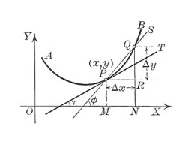
\includegraphics[height=5cm,width=5cm]{derivative_geometry.eps}
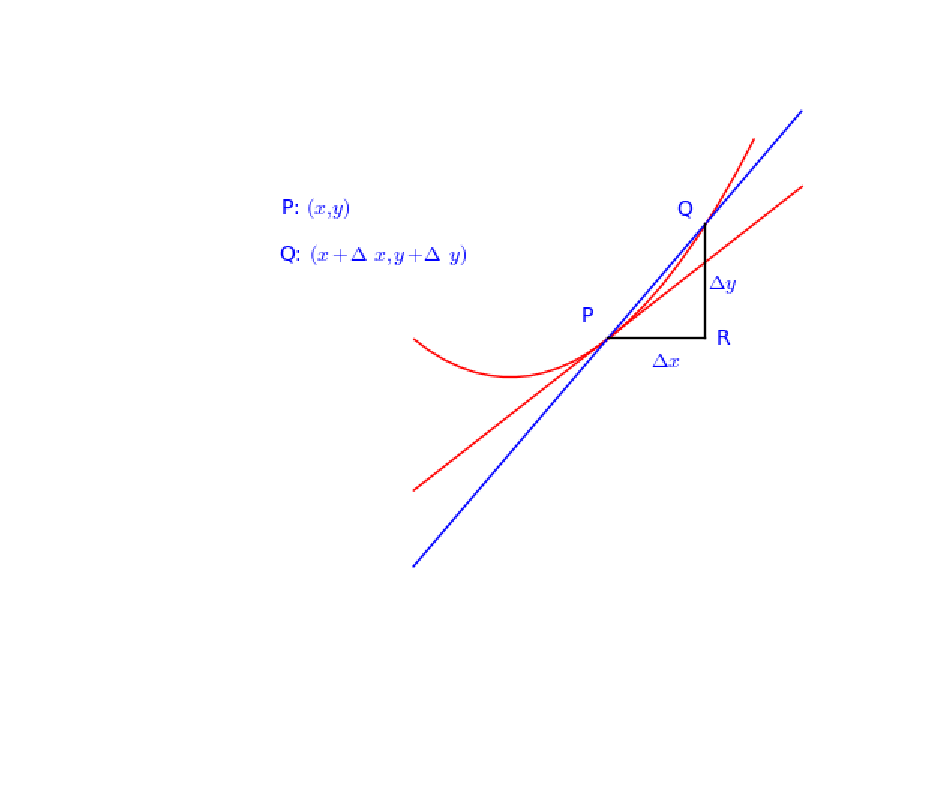
\includegraphics[height=6cm,width=8cm]{parabola-tangent.eps}
\end{center}
\end{minipage}
\caption{The geometry of derivatives.}
\label{fig:dg}
\end{figure}
%sage: p = plot(1+(x-1)^2, 0.5,2.25, rgbcolor=(1,0,0))
%sage: p1 = plot(x-1/4, 0.5, 2.5, rgbcolor=(1,0,0))
%sage: p2 = plot(3*x/2-1, 0.5, 2.5, rgbcolor=(0,0,1))
%sage: t1 = text('P', (1.4, 1.4))
%sage: t2 = text('Q', (1.9, 2.1))
%sage: t3 = text('$\Delta x$', (1.8, 1.1))
%sage: t4 = text('$\Delta y$', (2.1, 1.6))
%sage: t5 = text('P: $(x,y)$', (0.0, 2.1))
%sage: t6 = text('Q: $(x+\Delta\, x,y+\Delta\, y)$', (0.3, 1.8))
%sage: t7 = text('R', (2.1, 1.25))
%sage: P1 = line([(2,2),(2,5/4)], rgbcolor=(0,0,0))
%sage: P2 = line([(3/2,5/4),(2,5/4)], rgbcolor=(0,0,0))
%sage: show(p+p1+p2+t1+t2+t3+t4+t5+t6+t7+P1+P2,axes=False)

Let

\begin{equation}
%(A) 
y = f(x)
\label{eqn:A-32}
\end{equation}
be the equation of a curve $AB$.

Now differentiate (\ref{eqn:A-32}) by the General Rule and interpret each step geometrically.

\begin{itemize}
\item
FIRST STEP. $	y + \Delta y 	= f(x + \Delta x) 	= NQ$

\item
SECOND STEP. 
\[
\begin{array}{ll}
y + \Delta y &	= f(x + \Delta x) 	= NQ\\
  	y &	= f(x) 	= MP = NR\\
  	\Delta y &=	f(x + \Delta x) − f(x) 	= RQ.
\end{array}
\]

\item
THIRD STEP. 
\[
\begin{array}{ll}
\frac{\Delta y}{\Delta x} &	= \frac{f(x + \Delta x) - f(x)}{\Delta x} = \frac{RQ}{MN} = \frac{RQ}{PR}\\
&  	= \tan RPQ = \tan \phi \\
&  	= {\rm slope\ of\ secant\ line\ } PQ.
\end{array}
\]

\item
FOURTH STEP. 
\[
\begin{array}{ll}
	\lim_{\Delta x \to 0} \frac{\Delta y}{\Delta x} 
&= \lim_{\Delta x \to 0} \frac{f(x + \Delta x) - f(x)}{\Delta x}\\
%(B)
& 	= \frac{dy}{dx} = {\rm value\ of\ the\ derivative\ at\ } P.
\end{array}
\]
\end{itemize}

But when we let $\Delta x \to 0$, the point $Q$ will move along the curve 
and approach nearer and nearer to $P$, the secant will turn about $P$ and 
approach the tangent as a limiting position, and we have also

\[
\begin{array}{ll}
  	\lim_{\Delta x \to 0} \frac{\Delta y}{\Delta x} &= \lim_{\Delta x \to 0} \tan \phi = \tan \tau\\
%(C)
&  	= {\rm slope\ of\ the\ tangent\ at\ } P.
\end{array}
\]
Hence %from (B) and (C)
, $\frac{dy}{dx}$ = slope of the tangent line $PT$. Therefore

\begin{theorem}
The value of the derivative at any point of a curve is equal to the 
slope of the line drawn tangent to the curve at that point.
\end{theorem}

It was this tangent problem that led Leibnitz\footnote{Gottfried Wilhelm 
Leibnitz (1646-1716) was a native of Leipzig. 
His remarkable abilities were shown by original investigations 
in several branches of learning. 
He was first to publish his discoveries in Calculus in 
a short essay appearing in the periodical Acta Eruditorum at 
Leipzig in 1684. It is known, 
however, that manuscripts on Fluxions written by Newton were already 
in existence, and 
from these some claim Leibnitz got the new ideas. The decision of 
modern times seems 
to be that both Newton and Leibnitz invented the Calculus independently 
of each other. 
The notation used today was introduced by Leibnitz. See frontispiece.} 
to the discovery of the Differential Calculus.

\begin{example}
{\rm
Find the slopes of the tangents to the parabola $y = x^2$ at the vertex, 
and at the point where $x = \frac{1}{2}$.

Solution. Differentiating by General Rule, %p. 29 [§ 31]
(\S \ref{sec:31}), we get

\[
%(A)   
y' = \frac{dy}{dx} = 2x = {\rm slope\ of\ tangent\ line\ at\ any\ point\ on\ curve}.
\]

\begin{figure}[h!]
\begin{minipage}{\textwidth}
\begin{center}
%\vspace{1.0 cm}
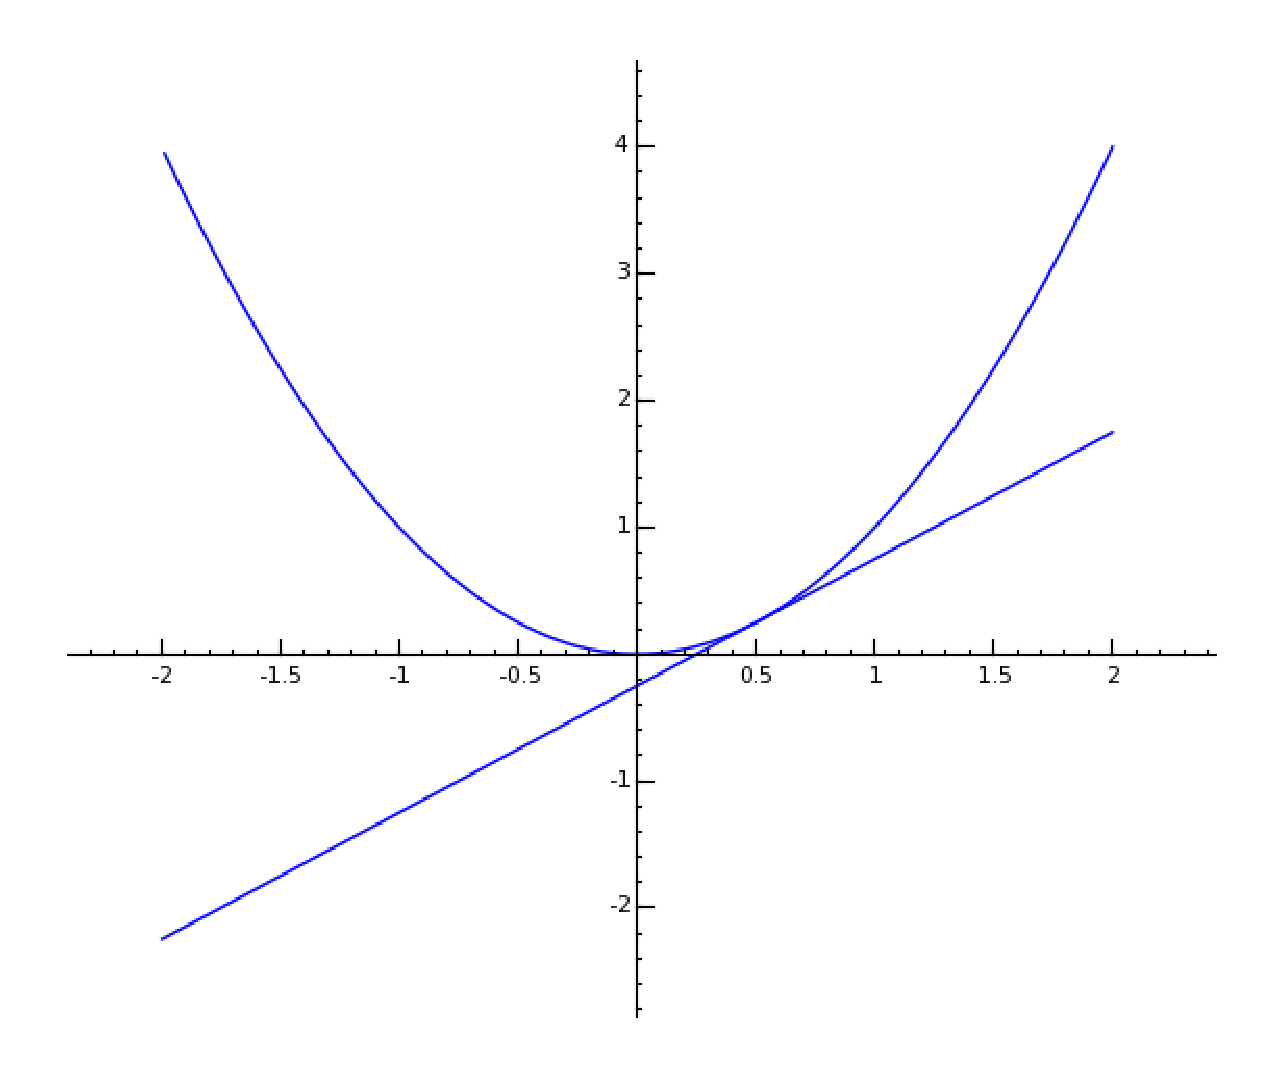
\includegraphics[height=8cm,width=4cm]{deriv-x2.eps}
\end{center}
\end{minipage}
\caption{The geometry of the derivative of $y=x^2$.}
\label{fig:x2}
\end{figure}
%sage: P1 = plot(x^2,-2,2)
%sage: P2 = plot(x-1/4,-2,2)
%sage: show(P1+P2)

To find slope of tangent at vertex, substitute $x = 0$ in %(A)
$y'=2x$, giving

\[
    \frac{dy}{dx} = 0.
\]
Therefore the tangent at vertex has the slope zero; that is, it is 
parallel to the axis of 
$x$ and in this case coincides with it.

To find slope of tangent at the point $P$, where $x = \frac{1}{2}$, 
substitute in %(A)
$y'=2x$, giving

\[
    \frac{dy}{dx} = 1;
\]
that is, the tangent at the point $P$ makes an angle of $45^o$ with 
the axis of $x$.
}
\end{example}

\section{Exercises}

Find by differentiation the slopes of the tangents to the following curves at 
the points indicated. Verify each result by drawing the curve and its tangent.

\begin{enumerate}

\item
%1. 
$y = x^2 - 4$, 	where $x = 2$. (Ans. $4$.)

\item
%2. 
$y = 6 − 3x^2$ where $x = 1$. (Ans. 	$-6$.)

\item
%3. 
$y = x^3$, 	where $x = -1$.  (Ans. $-3$.)

\item
%4. 
$y = \frac{2}{x}$, 	where $x = -1$. (Ans. $-\frac{1}{2}$.)

\item
%5. 
$y = x - x^2$, 	where $x = 0$. (Ans. $1$.)

\item
%6. 
$y = \frac{1}{x - 1}$, 	where $x = 3$. (Ans. $-\frac{1}{4}$.)
\item
%7. 
$y = \frac{1}{2} x^2$, 	where $x = 4$. (Ans. $4$.)

\item
%8. 
$y = x^2 - 2x + 3$, 	where $x = 1$. (Ans. $0$.)

\item
%9. 
$y = 9 − x^2$, 	where $x = -3$. (Ans. $6$.)

\item
%10. 
Find the slope of the tangent to the curve $y = 2x^3 - 6x + 5$, 
(a) at the point where $x = 1$; (b) at the point where $x = 0$.

(Ans. (a) $0$; (b) $-6$.)

\item
%11. 
(a) Find the slopes of the tangents to the two curves $y = 3x^2 - 1$ and 
$y = 2x^2 + 3$ at their points of intersection. (b) At what angle 
do they intersect?

(Ans. (a) $\pm 12$, $\pm 8$; (b) $\arctan \frac{4}{97}$.)

\noindent
{\small{
Here's how to use \sage to verify these:

\vskip .2in

\begin{Verbatim}[fontsize=\scriptsize,fontfamily=courier,fontshape=tt,frame=single,label=\sage]

sage: solve(3*x^2 - 1 == 2*x^2 + 3,x)
[x == -2, x == 2]
sage: g(x) = diff(3*x^2 - 1,x)
sage: h(x) = diff(2*x^2 + 3,x)
sage: g(2); g(-2)
12
-12
sage: h(2); h(-2)
8
-8
sage: atan(12)-atan(8)
atan(12) - atan(8)
sage: atan(12.0)-atan(8.0)
0.0412137626583202
sage: RR(atan(4/97))
0.0412137626583202

\end{Verbatim}

\vskip .1in
\noindent
}}

\item
%12. 
The curves on a railway track are often made parabolic in form. 
Suppose that a track has the form of the parabola $y = x^2$ 
%(last figure, p. 32 [§ 32])
(see Figure \ref{fig:x2} in \S \ref{sec:32}), 
the directions $OX$ and $OY$ being east and north respectively, and the unit of 
measurement $1$ mile. If the train is going east when passing through $O$, 
in what direction will it be going

\begin{itemize}
\item[(a)] 
when $\frac{1}{2}$ mi. east of $OY$? 	(Ans. Northeast.)

\item[(b)] 
when $\frac{1}{2}$ mi. west of $OY$? 	(Ans. Southeast.)

\item[(c)] 
when $\frac{\sqrt{3}}{2}$ mi. east of $OY$? 	(Ans. N. $30^o$E.)

\item[(d)] 
when $\frac{1}{12}$ mi. north of $OX$? 	(Ans. E. $30^o$S., or E. $30^o$N.)
\end{itemize}

\item
%13. 
A street-car track has the form of the cubic %al parabola 
$y = x^3$. 
Assume the same directions and unit as in the last example. If a car is going 
west when passing through $O$, in what direction will it be going

\begin{itemize}
\item[(a)] 
when $\frac{1}{\sqrt{3}}$ mi. east of $OY$? (Ans. Southwest.)
\item[(b)] 
when $\frac{1}{\sqrt{3}}$ mi. west of $OY$? (Ans. Southwest.)
\item[(c)] 
when $\frac{1}{2}$ mi. north of $OX$? (Ans. S. $27^o$ $43'$ W.)
\item[(d)] 
when $2$ mi. south of $OX$?
\item[(e)] 
when equidistant from $OX$ and $OY$?
\end{itemize}
\end{enumerate}

